\section{Evaluation}
 We present the basic statistics of our dataset in the first part, and then we evaluate the accuracy of our alignment and annotation process to ensure their reliability. Additionally, we not only test our dataset on different advanced models but also do ablation experiment on both modality and relations annotation. To discover interesting topics about personality dynamics, we focus on those changes of personality and discover several interesting psychological phenomenons.

\subsection{Dataset Statistics}

As we mentioned before, PersonaMovs is not only a large dataset containing a huge amount of text, audio and video corpus but also its data is highly diverse in terms of personality types, movie and television production genres, and relationship types. Fig \ref{Fig:Relats} are the distribution of two types of relations, which indicates the diversity in terms of interaction scenarios.

\begin{figure}[ht]
    \centering
    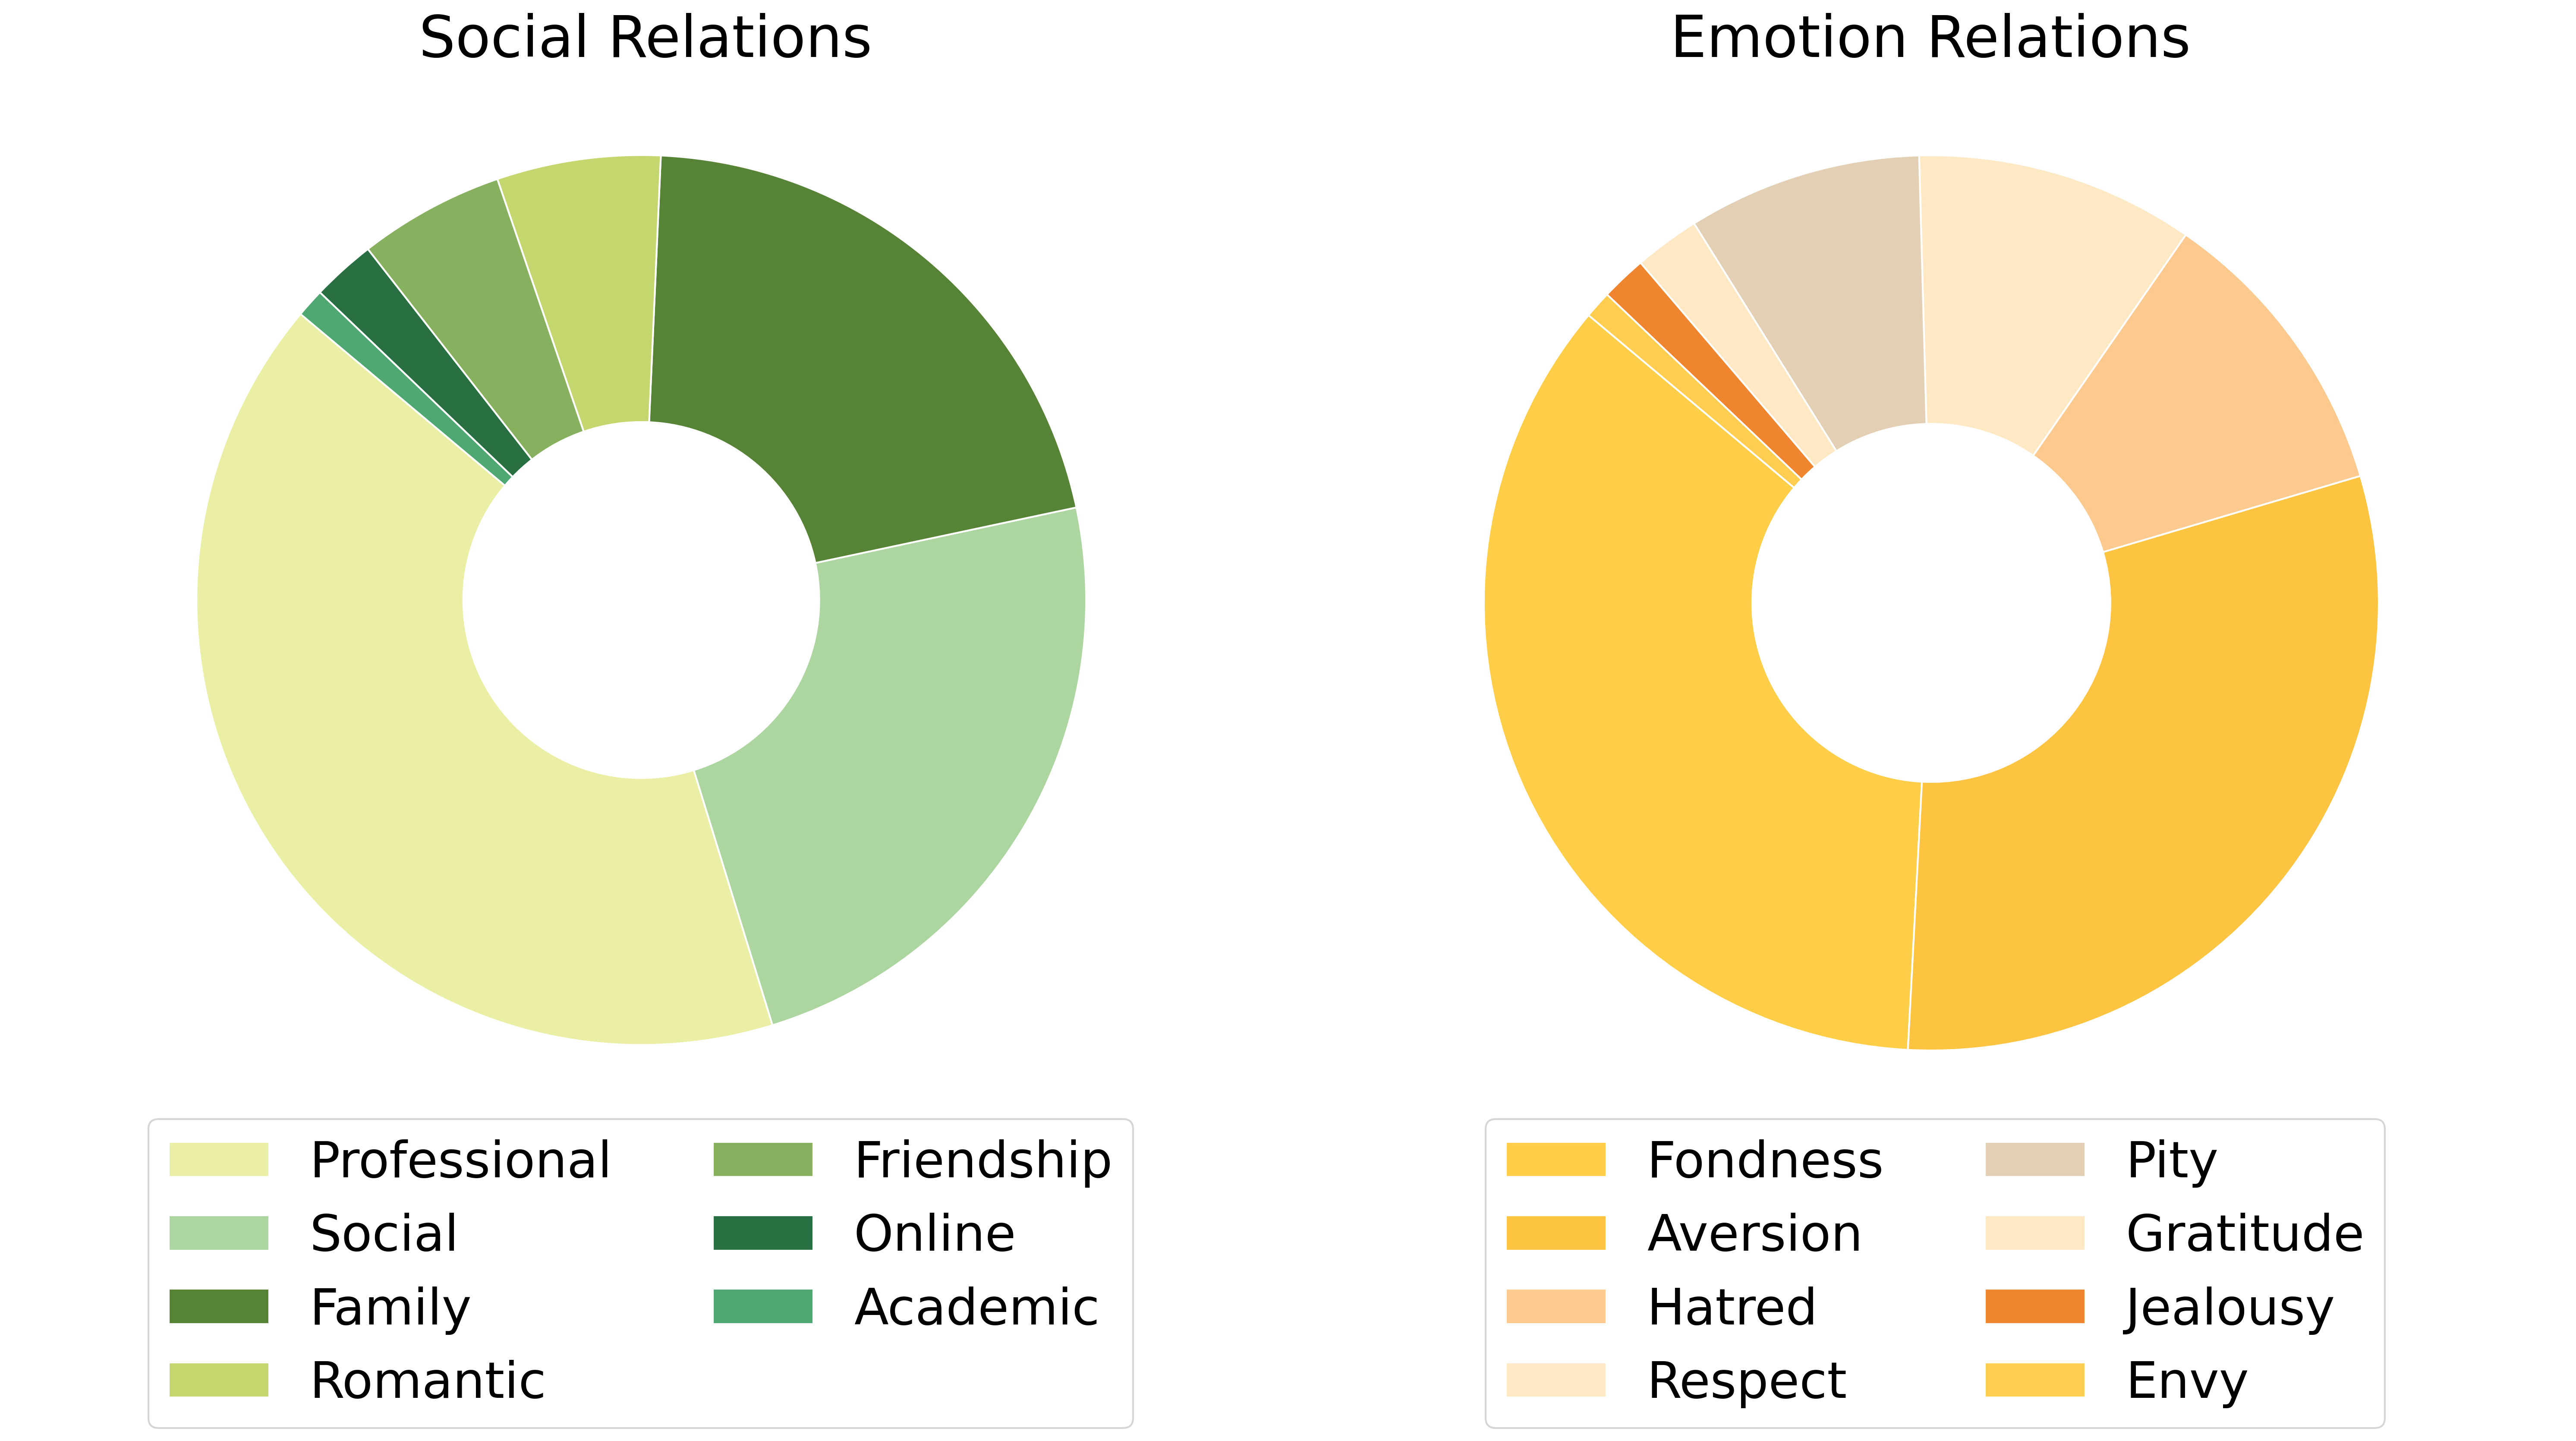
\includegraphics[width=0.75\linewidth]{images/relations.png}
    \caption{Distribution of social and emotion relations}
    \label{Fig:Relats}
\end{figure}


\subsubsection{Algorithm Evaluation}

To evaluate the performance of our character-to-subtitle matching algorithm, we manually check the aligned characters' name based on the script. The annotators were a group of five human volunteers with backgrounds in filmography and literary. They are in their mid-twenties and had at least an undergraduate education. The protocol involves the following steps: 1. Annotators independently reviewed a randomly selected sample of 50 dialogues from the dataset. By given relevant scripts and subtitle files, they are required to match each utterance in subtitle with corresponding names. 2. The annotations were compared against the results generated by our algorithm to evaluate accuracy. The algorithm demonstrates an accuracy of about 88\%, indicating a high level of accuracy in correctly identifying character names within subtitles across diverse content types. Compared to existing ASR matching algorithm, our approach gains an improvement by 5\% in accuracy. Besides, our algorithm shows a very strong efficiency comparing the ASR method, of which accelerating almost 7 times.

\begin{table}[ht]
    \small
    \centering
    \begin{tabular}{lllc}
        \hline
        \textbf{Method} & \textbf{Movies} & \textbf{TV} & \textbf{Exec. Time (s)}\\
        \hline
        Gentle (ASR) & 82.71\% & 85.21\% & 26.51\\
        \hline
        Our algorithm & 87.53\% & 88.98\% & 3.55\\
        \hline
    \end{tabular}
    \caption{Accuracy and running time per dialogue of subtitle matching algorithm}
\label{table:alg_eval}
\end{table}

\subsubsection{Annotation Accuracy}
Using ChatGPT to annotate relations for the characters is not a completely worthwhile method. To measure the automatic annotation accuracy, we sampled 235 scenes randomly and involved 5 human labelers on relations annotation. These labelers are in their mid-twenties, 
undergraduate or higher education background, proficient in English with majors in psychology, filmography and sociology, who were instructed to select one of the designated social and emotion relations after aligned video. We continue to compare the automatically annotated results to the human-labeled ground truth. The outcome shows that both social and emotional relationship annotations are dependable, with the accuracy reaching 95\% and 84\% respectively.

\begin{table}[ht]
    \centering
    \small
    \begin{tabular}{llll}
        \hline
        \textbf{Task} & \textbf{Movies} & \textbf{TV} & \textbf{Total}\\
        \hline
        Social Relations& 98.21\% & 93.91\% & 95.78\%\\
        \hline
        Emotion Relations& 82.04\% & 84.46\% & 84.01\%\\
        \hline
    \end{tabular}
    \caption{Accuracy of relations annotation.} 
\label{table:annota_eval}
\end{table}

The dataset's foundation on crowdsourced voting allows for an in-depth analysis of subjective biases in personality perception. Researchers can investigate how different demographics (age, gender, cultural background) perceive personality traits and emotions in characters, revealing biases that may exist in personality assessment. This could also extend to studying the impact of viewer's own personality traits on their perceptions of characters, thus contributing to a deeper understanding of projection and identification processes in media consumption.

\subsection{Experiment Results}
\subsubsection{Dataset Difficulties}
We test our dataset on popular models including BERT~\cite{devlin2019bert}, D-DGCN~\cite{yang2023orders}, Roberta~\cite{liu2019roberta}, AttRCNN~\cite{article1}, GPT-3.5~\cite{openai2023gpt35}, GPT-4~\cite{GPT-4-0125} and MCT~\cite{10386376}. We use the MBTI framework, which includes 16 distinct personality types, as the labels for our dataset. As shown in \tabref{table:Method_Comparison}, the accuracy of our dataset is lower than that of other comparable datasets. Accuracy here refers to the proportion of correctly predicted personality types out of the total number of predictions. One of the key challenges contributing to this lower accuracy is the increased complexity and diversity of our dataset, which encompasses a broader range of multimedia content compared to other datasets. 


\begin{table}[ht]
    \centering
    \small
    \begin{tabular}{lllll}
        \hline
        \textbf{Method} & \textbf{Modalities} & \textbf{FP} & \textbf{TVQA} & \textbf{PM} \\
        \hline
        BERT & T only& 61.14 & 60.61 & \textbf{52.94} \\
        \hline
        D-DGCN & T only & 69.56 & 70.21 & \textbf{68.47} \\
        \hline
        Roberta& T only &62.58 & 69.24 & \textbf{60.37} \\
        \hline
        AttRCNN & T only& 65.01 & 67.25 & \textbf{62.44}\\
        \hline
        GPT-3.5 & T only & 69.21 & 66.89 & \textbf{64.08}\\
        \hline
        GPT-4 & T \& V & 79.14 & 78.33 & \textbf{76.90}\\
        \hline
        MCT & T, A \& V & 71.67 & 69.93 & \textbf{68.47} \\
        \hline
    \end{tabular}
    \caption{Accuracy of different methods on Friends Persona (FP), TVQA, and PersonaMovs (PM). T, A, \& V stand for text, audio and video respectively. Lowest accuracy in each row is bolded.} 
\label{table:Method_Comparison}
\end{table}
A more challenging dataset, such as the one we have developed, offers several advantages in terms of personality detection: 1) Our dataset captures a wide range of real-life situations and intricate contexts, which better mirrors the complexity of human interactions. This realism is crucial for developing models that can perform well in practical applications. 2) Training on a more difficult dataset forces models to learn more nuanced patterns and relationships, leading to better generalization capabilities. 3) A difficult dataset sets a high standard for model evaluation, ensuring that only the most effective models are considered successful. This helps in distinguishing truly advanced models from those that perform well only on simpler tasks. Additionally, one notable observation from the results is that the MCT model, which leverages three modalities (text, audio, and video), does not outperform the GPT-4 model, which uses only two modalities (text and video). This performance gap suggests that Large Language Model outperforms the small model on this task, even though the latter uses more modalities.
\subsubsection{The Importance of Multi-Modality}



We conducted a series of ablation experiments to assess the impact of different modalities and relations annotations on the performance of personality prediction models. The experiments were designed to understand how the exclusion of specific modalities or relations annotations affects the overall prediction accuracy.

\begin{table}[ht]
    \small
    \centering
    \begin{tabular}{c|c|c}
        \hline
        \textbf{Method} & \textbf{Modality} & \textbf{Accuracy}\\
        \hline
        \multirow{4}{*}{MCT} & T \& A & 66.13  \\
        & T \& V & 67.91 \\
        & T only & 63.43 \\
        & T, A \& V & 68.47 \\  
        \hline
        \multirow{2}{*}{GPT-4-0125} & T only & 70.20 \\     
        & T \& V & 76.90 \\
        \hline
    \end{tabular}
    \caption{Ablation experiment on different modalities} 
\label{table:Ablation_modal}
\end{table}


Table \ref{table:Ablation_modal} presents the results of ablation experiments where different combinations of video and audio modalities were excluded. The result underscore the critical importance of using multiple modalities to achieve higher accuracy in personality prediction tasks. Models that leverage both audio and video data, in addition to text, consistently outperform those that rely solely on textual data. 
\begin{table}[ht]
    \centering
    \small
    \begin{tabular}{ccc}
        \hline
        \textbf{Method} & \textbf{With Relations} & \textbf{Without Relations} \\
        \hline
        BERT & 53.88 & 52.94 \\
        \hline
        Roberta & 59.21 & 58.39 \\
        \hline
        GPT-4-0125 & 73.22 & 70.20 \\  
        \hline
    \end{tabular}
    \caption{Ablation experiment on relations annotations.}
    \label{table:Ablation_relationship}
\end{table}

Table \ref{table:Ablation_relationship} shows the results of ablation experiments focusing on the inclusion or exclusion of relations' annotations which finds the relations annotations tend to slightly enhance the performance. This highlights the importance of including rich contextual information to improve the accuracy of personality prediction models. 


The multimodal nature of the dataset enables comprehensive studies that integrate different data types to understand personality. This could lead to the development of new theories or the refinement of existing ones that account for the complexity of personality as depicted through various media. It could also foster interdisciplinary research, combining insights from psychology, computer science, linguistics, and media studies.


\subsubsection{Personality Dynamics}
As mentioned in the Introduction, personality can change depending on various contexts. To explore this, we studied the relationship between the diversity of personalities and prediction accuracy. For each character, we calculate the entropy of the vote distribution to represent the personality dynamics as well as predicting their personalities using GPT-3.5. 

Entropy, denoted as \( H(X) \), is a measure of the uncertainty or complexity in a probability distribution. It is calculated using the formula:

\[
H(X) = - \sum_{i=1}^{n} p(x_i) \log_b(p(x_i))
\]

where \( X \) is a random variable representing the personality distribution, \( p(x_i) \) is the probability of each personality type \( x_i \), and \( b \) is the base of the logarithm, typically 2 when measuring entropy in bits. 

Figure \ref{fig:scatter} shows that as the complexity of a character's personality increases, the corresponding prediction accuracy decreases. This finding suggests that personality should be considered a dynamic attribute rather than a static one.

\begin{figure}
    \centering
    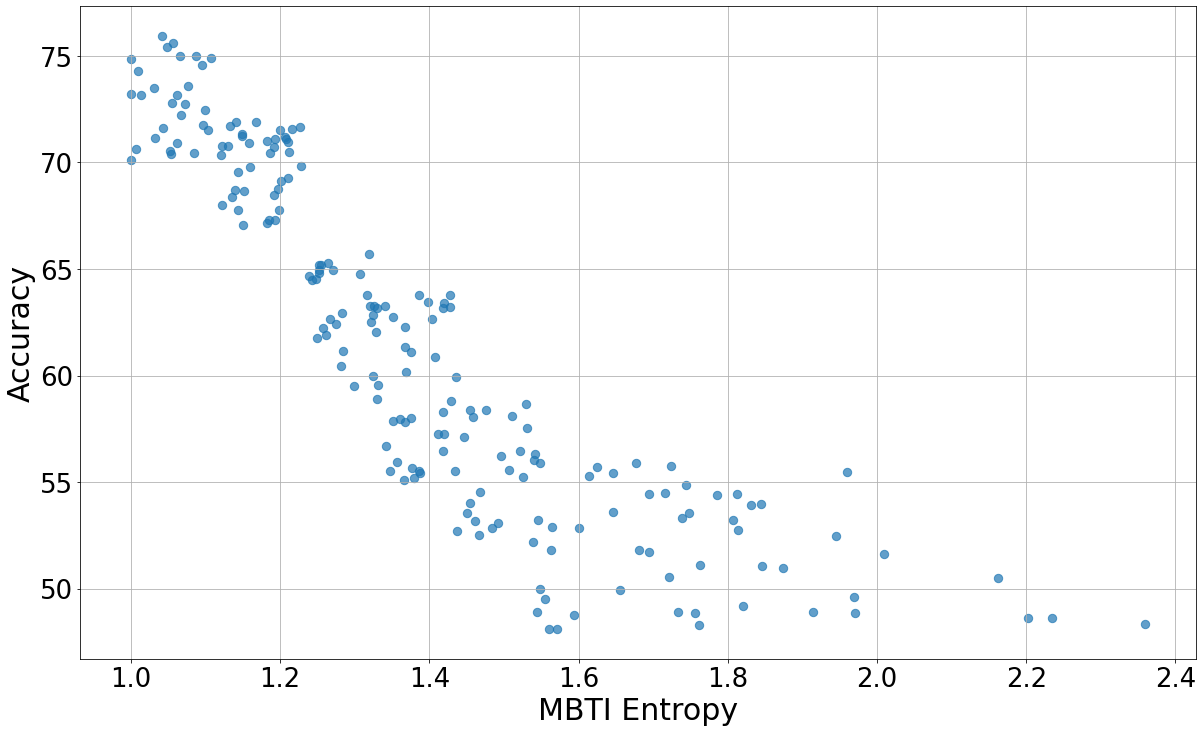
\includegraphics[width=\linewidth]{images/Scatter.png}
    \caption{Relationship between MBTI entropy and prediction accuracy}
    \label{fig:scatter}
\end{figure}

To solve this concern, movies and TV series and their characters often evolve over time, offering a fertile ground for studying personality dynamics. The dataset allows for longitudinal studies on how characters' personalities change in response to narrative events, relationships, and challenges. This could lead to new models that explain personality development and dynamics in complex social settings, bridging narrative theory and psychological research. 

We select two famous characters to find their potential change of personality, and we discover there are two types of personality shifts. In the short term, people show different personalities depending on their relations with interlocutor. For example, as shown in Figure \ref{fig:dynamics}, Jay Gatsby from the famous romantic movie ``\textit{The Great Gatsby}'' behaves as an INFJ in front of his beloved Daisy and as an ENFJ in front of his business partners. In the long term, people may change their personality due to major turning point of life. Like Mia Dolan in ``\textit{La La Land}'', she was always ENFJ, but after the breakup she became an ISFJ. The prediction results generated by GPT-4 align with the peaks in the voting distribution, indicating that this personality shift is observable within our realistic dataset.

According to our finding, we conduct statistical analysis based on our dataset to figure out if there exists certain personalities that are easily attracted to each other. To analyze the patterns of personality attraction, we focus on identifying pairs of personalities that frequently appear together bi-directionally in fondness, aversion, romantic and friendship relations. Figure \ref{fig:networks} presents the favorite network with 16 MBTI personality types, providing a clear visual summary of statistical findings. The size of each node is proportional to the number of connections (degree) it has, which means personality types with more relationships are represented by larger nodes. The color of the edges represents the weight of the relationship between the personality types. Darker edges indicate a higher frequency or stronger relationship. 
%Based on these vivid figures, we can discover very interesting psychological phenomenons. 
For instance, ISTP is the most popular personality since almost every other personality has a fondness relation with it, and ESTP prefers to be around ESFP, ENFP and people with the same personality as themselves. ESFP may not like people with same personality.
% because it has a dark circle on itself.
\begin{figure}[ht]
    \centering
    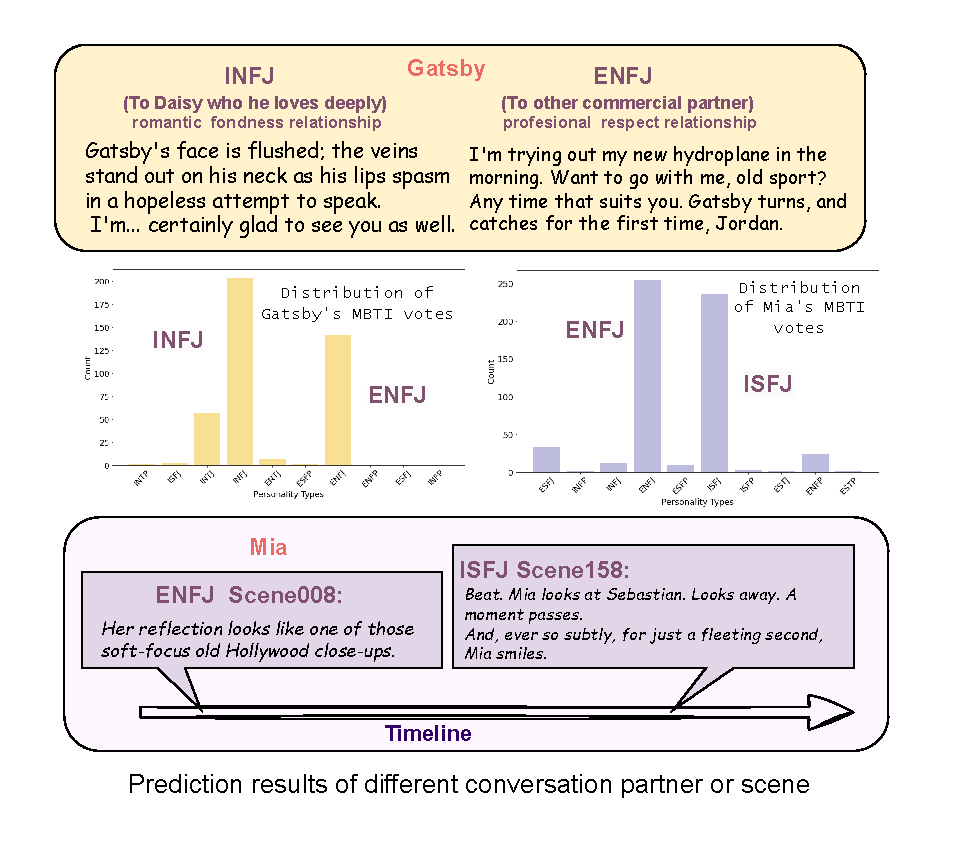
\includegraphics[width=\linewidth, trim= 0 10 0 0, clip]{images/Dynamics.pdf}
    \caption{Case study for personality dynamics.}
    \label{fig:dynamics}
\end{figure}

\begin{figure}[!h]
    \centering
    \begin{subfigure}[b]{0.22\textwidth} 
        \centering
        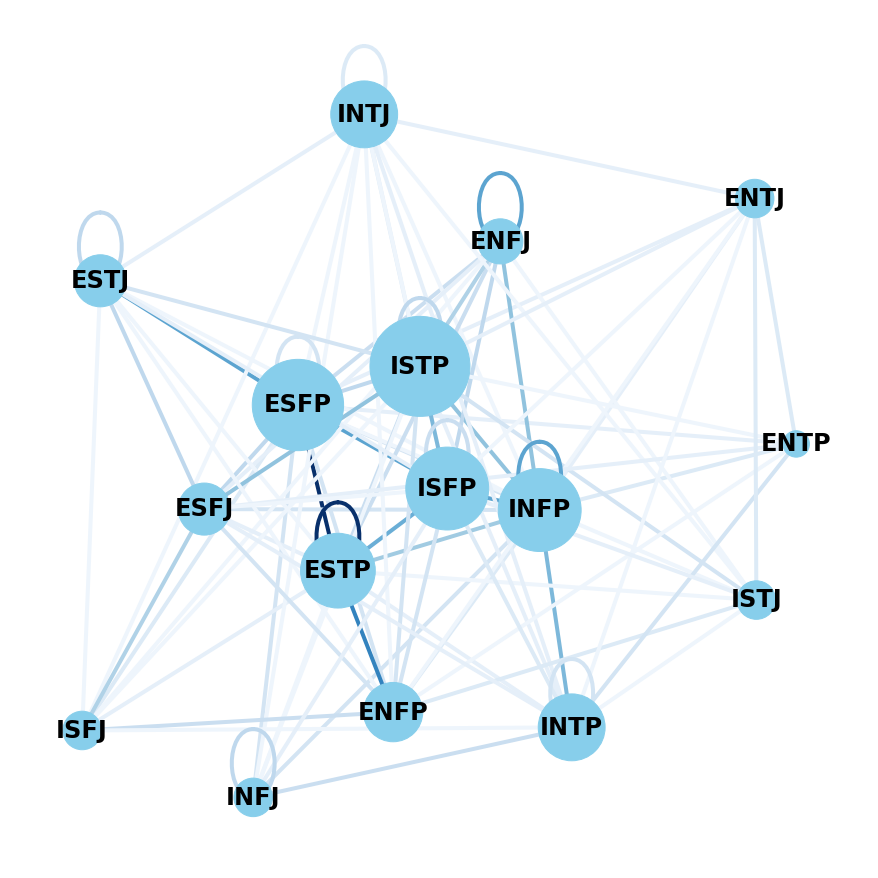
\includegraphics[width=\linewidth, scale=0.7]{images/fondness.png} 
        \caption{Fondness}
        \label{fig:subgraph1}
    \end{subfigure}
    \hfill
    \begin{subfigure}[b]{0.22\textwidth} 
        \centering
        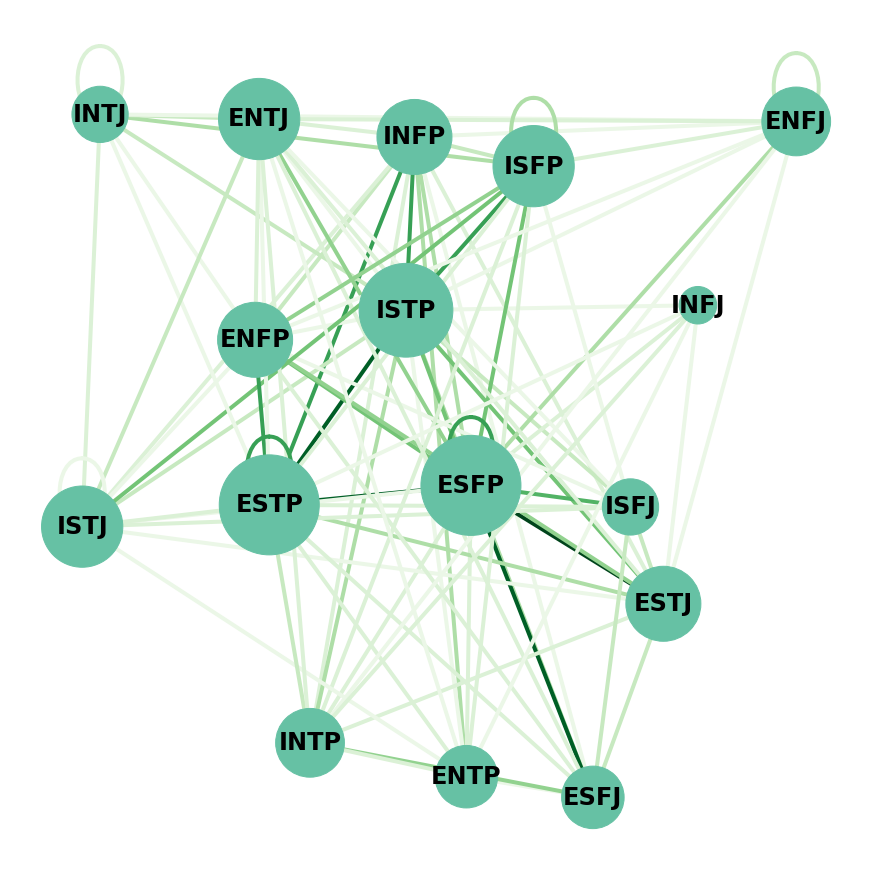
\includegraphics[width=\linewidth, scale=0.7]{images/dislike.png}
        \caption{Aversion}
        \label{fig:subgraph2}
    \end{subfigure}
    \hfill
    \begin{subfigure}[b]{0.22\textwidth} 
        \centering
        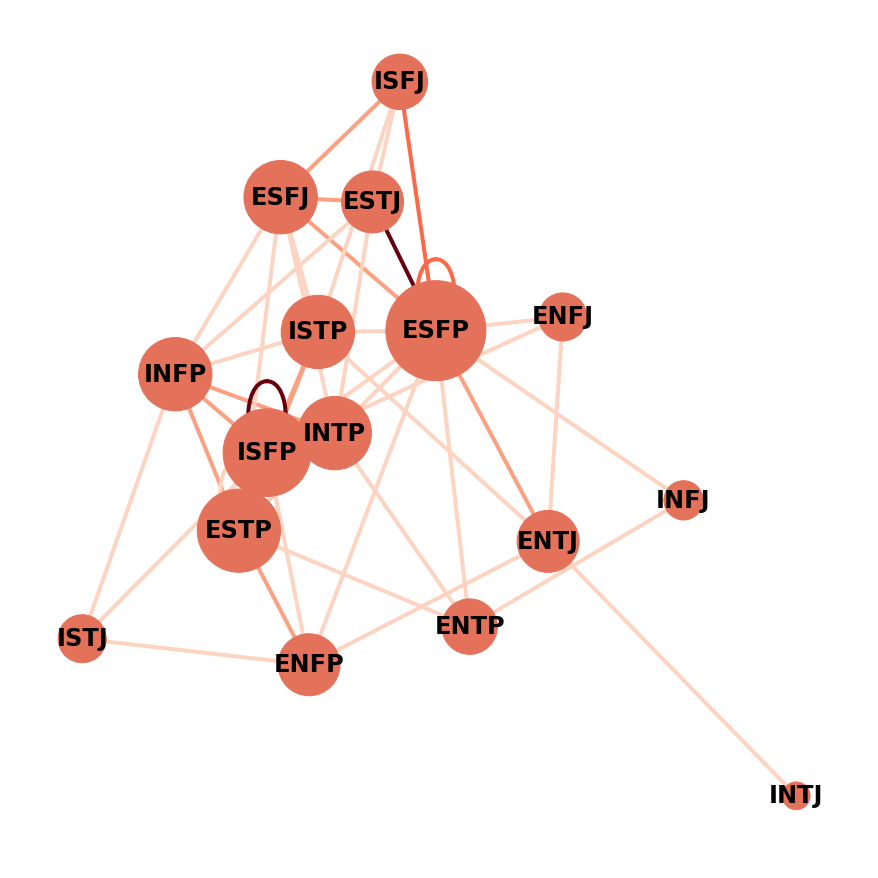
\includegraphics[width=\linewidth, scale=0.7]{images/romantic.png}
        \caption{Romantic}
        \label{fig:subgraph3}
    \end{subfigure}
    \hfill
    \begin{subfigure}[b]{0.22\textwidth} 
        \centering
        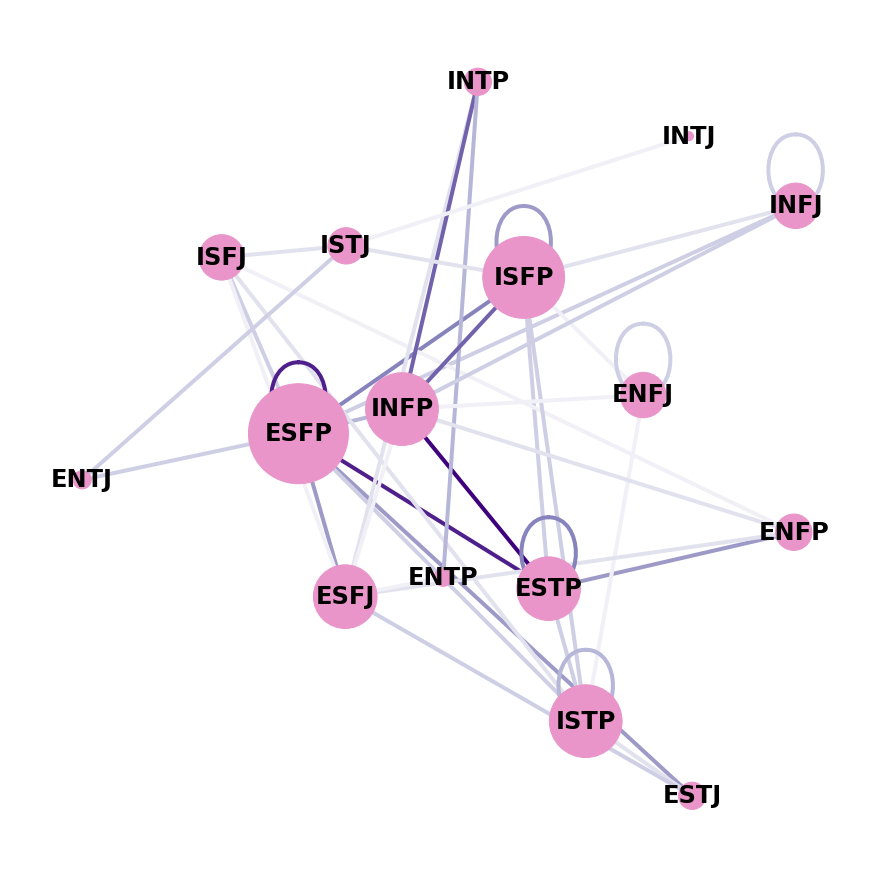
\includegraphics[width=\linewidth, scale=0.7]{images/friendship.png} 
        \caption{Friendship}
        \label{fig:subgraph4}
    \end{subfigure}
    \caption{Favorite Networks with Different Personalities about Four Relations}
    \label{fig:networks}
\end{figure}

By including data on social and emotion relations between characters, the dataset opens new pathways for exploring the dynamics of personality through interactions. This aspect provides a basis for computational models that simulate personality dynamics in social networks, potentially informing theories on social behavior, conflict resolution, and group dynamics.
